\documentclass[12pt]{article}
\usepackage{verbatim}
\usepackage[dvips]{epsfig}
\usepackage{color}
\usepackage{url}
\usepackage[colorlinks=true]{hyperref}

\begin{document}

\section*{GENESIS: Documentation}

{\bf Related Documentation:}
% start: userdocs-tag-replace-items related-do-nothing
% end: userdocs-tag-replace-items related-do-nothing

\subsection*{Source}

De Schutter E \& Bower JM (1994) An active membrane model of the cerebellar Purkinje cell I. Simulation of current clamp in slice. {\it Journal of Nerurophysiology}. {\bf 71}: 375--400. \\

\subsection*{A Current (KA)}

\begin{figure}[h]
\centering
   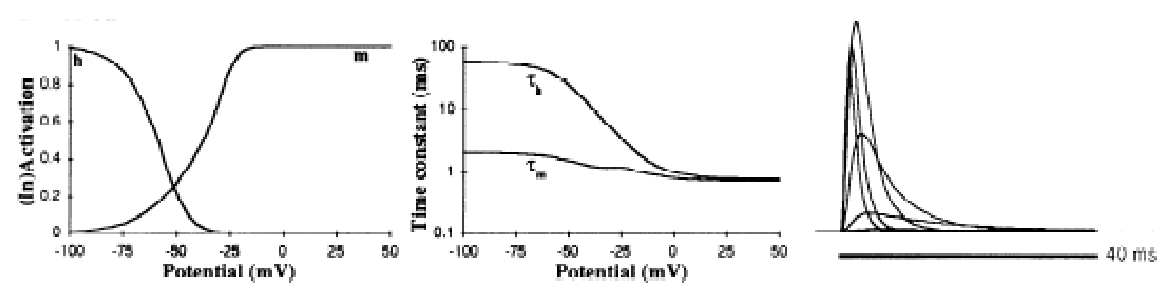
\includegraphics[scale=0.75]{figures/DS1.2F.eps}
   \caption{Activation and inactivation properties of the A current (Ka, ---) in the model. Seady-state activation and inactivation vs. voltage are plotted at the {\em left}, the time constants of activation and inactivation($\tau_m$ and $\tau_h$) vs. voltage in the {\em middle} (Note: Semilogarithmic scale), and a simulation of representative voltage-clamp currents at the {\em right}. The voltage clamps simulate steps from a holding potential of -110 to -70\,mV up to 0\,mV in 10\,mV increments. The voltage-clamp current amplitude has been scaled arbitrarily because we mainly wanted to demonstrate the current kinetics.}
   \label{fig:DS1.2F}
\end{figure}

The presence of a conductance like an A current (KA) in the Purkinje cell was shown by\,\cite{Hounsgaard:1988nx}. We derived our equations for KA from the original reports on A currents\,\cite{Connor:1971tg, De-Schutter:1986hc} modified to fit the data in the two reports on Purkinje cell A currents that were available at that time. The whole cell voltage-clamp study of cultured Purkinje cells by\,\cite{Hirano:1989uq} (their Fig. 9) provided data about the activation and inactivation time constants and the steady-state inactivation, and a single-electrode voltage-clamp study in slice by\,\cite{Li:1990ij} supplied steady-state activation data.

Recently\,\cite{Wang:1991bs} published a more complete report on a single-electrode voltage-clamp study of the Purkinje cell. The average threshold for activation they report is lower than the value used in our model, but there seems to be a large natural variability in the activation curves (compare their Fig. 1 with their Table 1). The steady-state inactivation curve of\,\cite{Wang:1991bs} is similar to ours and to the kinetics of A currents in other systems\,\cite{Connor:1971tg, Rogawski:1985fv} but they report a much slower inactivation time constant than\,\cite{Hirano:1989uq}.

\bibliographystyle{plain}
\bibliography{../tex/bib/g3-refs}

\end{document}
